\appendix
\pagenumbering{Roman}
\renewcommand{\thepage}{\Roman{page}}

\chapter{Algorithmes et Code}

\section{Opérations Logiques}
\label{app:logical_ops}
En \ref{subsubsec:enc}, nous avons vu comment encoder en pseudo-code un pion et un plateau.
\\ \\
\noindent \textbf{En Python :}
\begin{figure}[H]
    \centering
    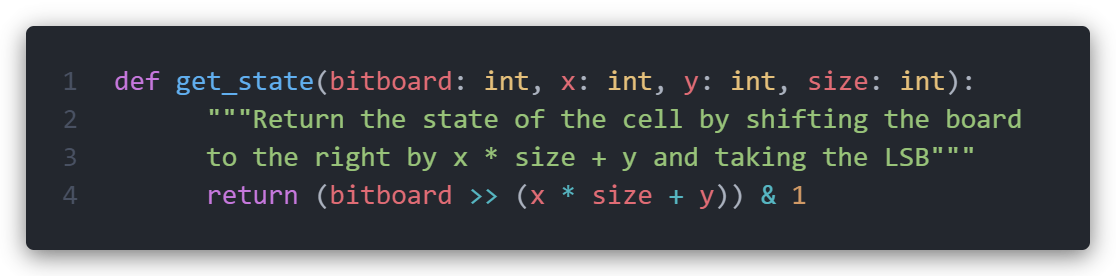
\includegraphics[width=1\textwidth]{ressources/get_state.png}
    \caption{Opérations logiques pour obtenir l'état du plateau.}
    \label{fig:get_state}
\end{figure}
\begin{figure}[H]
    \centering
    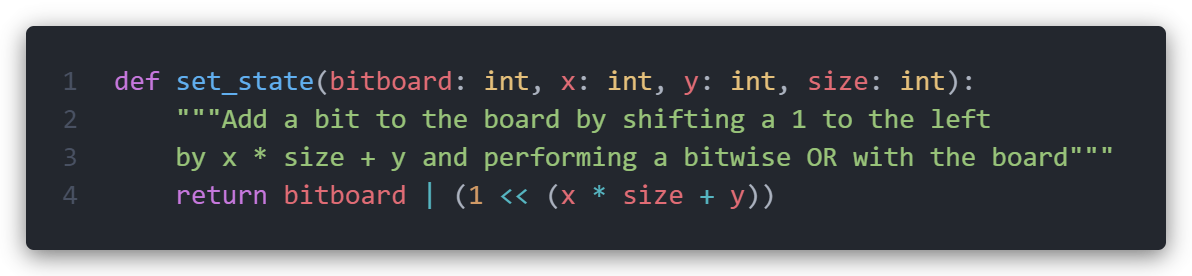
\includegraphics[width=1\textwidth]{ressources/set_state.png}
    \caption{Opérations logiques pour définir l'état du plateau.}
    \label{fig:set_state}
\end{figure}

En \ref{subsec:shift}, nous avons vu comment décaler un bitboard dans 4 directions cardinales. Voyons maintenant comment décaler un bitboard dans les 4 directions diagonales, et leur équivalent en python.

\begin{algorithm}[H]
    \caption{Opérations de décalage en diagonales.}
    \begin{algorithmic}[1]
    \Function{NordEst}{$x$}
        \State \Return $Nord(Est(x))$
    \EndFunction

    \Function{NordOuest}{$x$}
        \State \Return $Nord(Ouest(x))$
    \EndFunction

    \Function{SudEst}{$x$}
        \State \Return $Sud(Est(x))$
    \EndFunction

    \Function{SudOuest}{$x$}
        \State \Return $Sud(Ouest(x))$
    \EndFunction
    \end{algorithmic}
\end{algorithm}

\noindent \textbf{En Python :}
\begin{figure}[H]
    \centering
    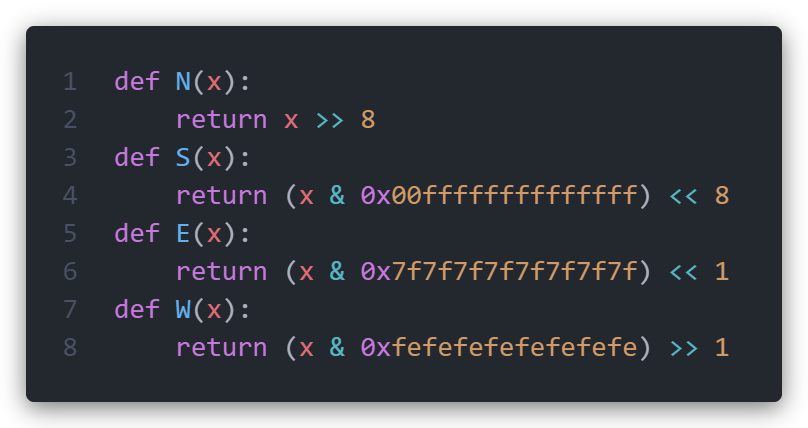
\includegraphics[width=0.7\textwidth]{ressources/operateurCardinaux.png}
    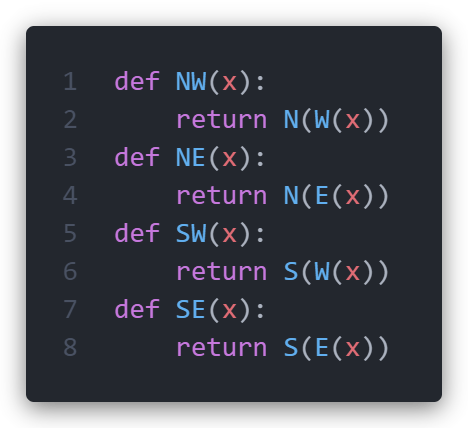
\includegraphics[width=0.5\textwidth]{ressources/operateurCardinauxComposes.png}
    \caption{Opérations de décalage pour les coups valides.}
    \label{fig:shift_ops}
\end{figure}